\documentclass[a4paper, 10pt, 
               numbers=noenddot, toc=graduated,
               headsepline=true, footsepline=true,
               twoside=false, titlepage=true, 
               bibliography=totoc]{scrartcl}



\usepackage[a4paper, top = 2.5cm,
  	bottom = 2.0cm,
    left   = 2.0cm,
    right  = 2.0cm]{geometry}

\usepackage{graphicx}
\usepackage{amsmath} %math package
\usepackage{amssymb}
\usepackage[font={footnotesize}, bf]{caption}
\renewcommand{\arraystretch}{1.2}

\usepackage{longtable}
\usepackage{lscape}
\usepackage{siunitx}	
%\usepackage{citesort} 

\usepackage[toc,page]{appendix}
\setlength\parindent{0pt}
\usepackage{subcaption}
\usepackage{cite} 
%\usepackage{float} 
\usepackage[utf8x]{inputenc}		% input encoding
\usepackage[ngerman]{babel} 
\captionsetup{format=plain}
\addto\captionsenglish{\renewcommand{\figurename}{Fig.}}
\addto\captionsenglish{\renewcommand{\tablename}{Tab.}}
\usepackage[T1]{fontenc}                % mathmode for font Palatino
%\usepackage[plainfootsepline ,autooneside]{scrpage2}	% header and footer for komascript
\usepackage{hyperref}
\usepackage[procnames]{listings}

\usepackage{url}
\usepackage{titling}
\usepackage{multirow}
 

\usepackage{floatrow}
% Table float box with bottom caption, box width adjusted to content
\newfloatcommand{capbtabbox}{table}[][\FBwidth]


\usepackage{array}

\makeatletter
\newcommand{\thickhline}{%
    \noalign {\ifnum 0=`}\fi \hrule height 1pt
    \futurelet \reserved@a \@xhline
}
\newcolumntype{"}{@{\hskip\tabcolsep\vrule width 1pt\hskip\tabcolsep}}
\makeatother

%\usepackage{fancyhdr}
%\pagestyle{fancy}
%\fancyhf{}
%\fancyheadoffset{0 cm}

%\rhead{\nouppercase\rightmark}
%\lhead{\thepage}

\newif\ifinternal

\internalfalse

\newcommand*\mean[1]{\overline{#1}}

\begin{document}

\title{Bestimmung der strahlungsinduzierten Viskosit{\"a}t mit Hilfe von LAMMPS}
\author{Christian Schleich, Alexander Toifl}

\begin{center}
\huge{\thetitle} \\
\small{\theauthor, \today}
\end{center}

%\tableofcontents
\hspace{1 cm}


\section{Strahlungsinduzierte und dynamische Viskosität}

Die im betrachteten Paper \cite{Mayr2003} beschreibene Methode wird in \cite{hobler2017hpm} schön zusammengefasst.

\begin{itemize}
	 \item Definition der Strahlungsinduzierten Fluidität $H = \frac 1 {\eta \dot{\phi}} = \frac 1 {\eta^{'}}$  ($\eta$ ... Viskosität, $\dot{\phi}$ ... 'flux', $\eta^{'}$ ... strahlungsind. Viskosität) \cite{Mayr2003}
\end{itemize}


\section{MD Methoden zur Bestimmung der Viskosität}

Allgemeine Informationen zum Aufschmelzen und Abkühlen (Temperatur und Druck) mit MD - Simulationen (in Ge - Dünnschichten) zur Amorphisierung des Materials finden sich in \cite{Mayr2005}. Außerdem werden auch Werte für die strahlungsinduzierte Viskosität in Abhängigkeit der Defektdichte dpa angegeben (Methode?). Ebenfalls wird dies in \cite{Edler2007} beschrieben, wobei hier aber nur mech. Stressbetrachtungen gemacht werden. In \cite{Lehnert2017} wird die in \cite{Mayr2003} erwähnte Methode auf a-Ge-Si Legierungen angewandt um mithilfe der Fluidität die Formierung von porösen Strukturen zu begründen.


\subsection{Non-equilibrium MD (NEMD) Simulationen}

System wird verformt (Scherung) und die resultierende Spannung wird ermittelt. 


	\subsubsection{SLLOD}
		\begin{itemize}
		 	\item Original Paper, indem SLLOD Dynamik vorgestellt werden \cite{Evans1984}
		 	\item Dem System wird eine Schergeschwindigkeit (shear rate) $\dot{\gamma}$ aufgezwungen. Als Folge ergibt sich ein Impulsfluss, der über die Nebendiagonalelemente des Spannungs- oder Drucktensors gemessen wird\cite{Tenney2010}.
		 	\item Problem: Druck variiert typischerweise sehr stark in MD Simulationen, daher ist die Konvergenz eher langsam\cite{Tenney2010}.
		 	\item LAMMPS: Simulationsbox wird geschert. Kombination von fix nvt/sllod und fix deform.
		\end{itemize}
		
	\subsubsection{Moving Walls}
	    \begin{itemize}
		 	\item LAMMPS: 'walls' werden definiert, eine ist ortfest, die zweite bewegt sich. Damit wird Scherung erreicht
		\end{itemize}

\subsection{Reverse Non-Equlibirium MD  (rNEMD) Simulationen}
	\begin{itemize}
		 \item Zusammenfassende Beschreibung in \cite{Tenney2010} 
		  \item \textbf{Impulsfluss} wird vorgegeben und die \textbf{Schergeschwindigkeit} (Geschwindigkeitsprofil) wird gemessen.
		  \item Vorteil: Schergeschwindigkeit ist leichter aus MD Simulationen zu ermitteln
		  \item Simulationsbox wird in N kline Kästchen entlang der z-Achse eingeteilt
		  \item Vorgabe der Schergeschwindigkeit: \textbf{Periodischer} Tausch von Momenten (momenta swaps) 
		  		\begin{itemize}
			  		\item Ursprüngliche Implementierung: x-Komponente des Impulses des Atoms mit der negativsten Impulskompentente in Kästchen 1 $p_{x,n_1}$ wird mit der x-Komplente des Atomes mit der positivsten Impulskomponente im Kästchen $n = n_c = N/2 + 1$, $p_{x,n_c}$ getauscht.
			  		\item Lammps-Implementierung: Eine Zielgeschwindigkeit $\pm v_{x,t}$ wird definiert. Impuls der beiden Atome, die jeweils am knappsten am positiven/negativen Wert liegt, wird getauscht.
		  		\end{itemize}
		  \item Da Gesamtimpuls und kinetische Energie erhalten bleiben, ist prinzipiell kein Thermostat nötig
		  \item Die Tauschfrequenz bestimmt den insgesamt ins System eingeprägten Impulsfluss.
		  \item Das System antwortet auf den unphysikalisch erzwungenden Fluss mit einem 'echten' Impulsfluss in die entgegengesetzte Richtung. Dadurch ergeben sich Geschwindigkeitsprofile in der oberen und unteren Hälfte der Simulationsbox.
		  
  		  \item Berechnung der Viskosität
  		  		 \begin{equation}
  		   		 	\eta = \frac{-j_{xz} }{\dot{\gamma} },\quad j_{xz} = \frac{p_{\mathrm{total}}}{2 t L_x L_y},\quad p_{\mathrm{total} }= \sum (p_{x,n_c} - p_{x,n_1})
  		   		\end{equation}
  		   
  		   $j_{xz}$ ... Eingeprägter Impulsfluss, $L_x,\,L_y$ ... Längen der Kästchen, $t$ ... Zeit\\
  		   $\dot{\gamma} = \frac{\mathrm{d}v_x}{\mathrm{dz}}$ ergibt sich aus der Geschwindigkeitsverteilung
		  
		 \item Setup der LAMMPS MD Simulationen von \cite{Tenney2010} 
		 		\begin{itemize}
		 			\item 3D orthogonale Simulationsbox
		 			\item Periodische RB
		 			\item Verlet Zeitschrittverfahren
		 			\item Equilibrisierung bei \SI{10}{K} mithilfe eines Berendesen Thermostats (kein Impulstausch findet statt)
		 			\item Simulationbox wird in 20 Kästchen entlang der z-Achse eingeteilt
		 			\item Impulstausch zwischen erster und mittlerer Box
		 			\item Tauschfrequenz: Nach jedem 1., 10., 100. Simulationszeitschritt
		 		\end{itemize}
		 	
		 
		 
		\begin{figure}[H]
	    	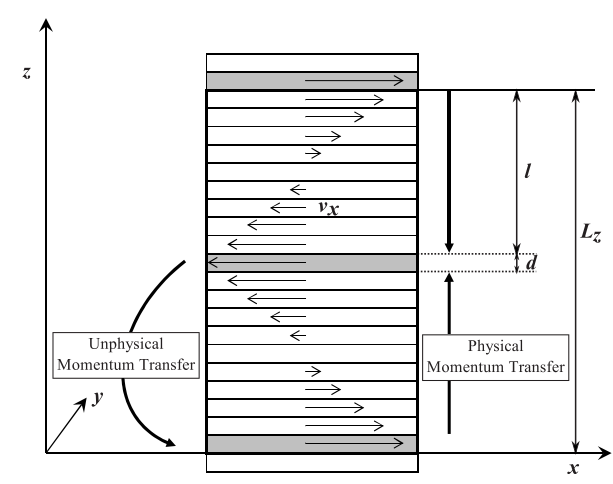
\includegraphics[width=0.4\textwidth]{figs/rnemd_box}%
	    	\caption{RNEMD simulation box \cite{Tenney2010}, Fig. 1.}
   		\end{figure}		 
		 
	\end{itemize}



\subsection{Autokorrelation des Drucktensors (Green-Kubo)}
	\begin{itemize}
		 \item Zusammenfassende Beschreibung \cite{Tenney2010}
		 \item Mathematische Formulierung  \cite{Tenney2010} (in Abschnitt EMD, eher minimal gehalten), \cite{Kirova2015} (etwas ausführlicher)
		 \item Bsp in LAMMPS verweist auf \cite{Daivis1994}
	\end{itemize}

\subsection{Einstein Formulierung der Green-Kubo Methode}
	\begin{itemize}
		 \item Zusammenfassende Beschreibung \cite{Tenney2010}
		 \item Mathematische Formulierung  \cite{Tenney2010} (in Abschnitt EMD)
	\end{itemize}

\section{Experimentelle Befunde}

\subsection{Stress und Viskositätsbetrachtungen}
	\begin{itemize}
		\item Betrachtungen für $SiO_2$ in \cite{Snoeks2000}
	\end{itemize}



\bibliographystyle{Citation/IEEEbib-c.bst}
\bibliography{Citation/MolecularDynamics}


\end{document}  
